\documentclass[11pt, letterpaper, notitlepage]{article} 
\usepackage[
    top=1in,
    left=0.75in,
    right=0.75in,
    bottom=1in,
    headheight=60pt,
    % showframe
]{geometry}
\usepackage[T1]{fontenc}
\usepackage{tgadventor}
\usepackage{titlesec}
\usepackage{fancyhdr}
\usepackage{lastpage}
\usepackage{tocloft}
\usepackage[fleqn]{amsmath}
\usepackage{amssymb}
\usepackage{multirow}
% \usepackage{float}
\usepackage{lscape} % For certain tables to be in landscape mode
% \usepackage{etoolbox}
\usepackage{enumitem}
\usepackage{multicol}
\usepackage{textcomp}
\usepackage{romannum}
\usepackage{graphicx}
\usepackage{float}
\usepackage{hyperref}
\hypersetup{
  colorlinks=true,
  linkcolor=black,
  filecolor=magenta,      
  urlcolor=blue,
}

\AtBeginDocument{\pagenumbering{arabic}}

\DeclareMathVersion{sans}
\SetSymbolFont{operators}{sans}{OT1}{cmbr}{m}{n}
\SetSymbolFont{letters}{sans}{OML}{cmbrm}{m}{it}
\SetSymbolFont{symbols}{sans}{OMS}{cmbrs}{m}{n}
\SetMathAlphabet{\mathit}{sans}{OT1}{cmbr}{m}{sl}
\SetMathAlphabet{\mathbf}{sans}{OT1}{cmbr}{bx}{n}
\SetMathAlphabet{\mathtt}{sans}{OT1}{cmtl}{m}{n}
\SetSymbolFont{largesymbols}{sans}{OMX}{iwona}{m}{n}

\title{MEEN 621 Notes}
\author{Shivanand P}

\titleformat{\section}[block]{\bfseries \sffamily \large}{\thesection.}{5pt}{}
\titleformat{\subsection}[block]{\bfseries \sffamily \normalsize}{\thesubsection.}{5pt}{}
\titleformat{\subsubsection}[block]{\bfseries \sffamily \small}{}{0pt}{}

\makeatletter
% \patchcmd{\LS@rot}{90}{-90}{}{}
% \patchcmd{\endlandscape}{90}{-90}{}{}
\newenvironment{mywideralign*}{\ifvmode\else\hfil\null\linebreak\fi
  \hspace*{-\leftmargin}\minipage\textwidth
  \setlength{\abovedisplayskip}{0pt}%
  \setlength{\abovedisplayshortskip}{\abovedisplayskip}%
  \start@align\@ne\st@rredtrue\m@ne}%
{\endalign\endminipage\linebreak}
\makeatother
\begin{document}

\sffamily
\sffamily\mathversion{sans}

\date{\vspace{-5ex}}
\maketitle
\renewcommand{\cftpartleader}{\cftdotfill{\cftdotsep}} % for parts
\renewcommand{\cftsecleader}{\cftdotfill{\cftdotsep}}
{ \hypersetup{linkcolor=black} \tableofcontents }
\thispagestyle{empty}

\newpage
\setcounter{page}{1}

\pagestyle{fancy}
\fancyhead{}    
\fancyhead[R]{\normalfont\sffamily Shivanand P \\ MEEN 621 Notes}
\fancyfoot{}
\fancyfoot[R]{\normalfont\sffamily Page \textbf{\thepage} of \textbf{\pageref{LastPage}}}
\renewcommand{\headrulewidth}{0pt}
\renewcommand{\footrulewidth}{0pt}
\renewcommand{\arraystretch}{1.75}

\newpage
\section{Mathematics}

\subsection{Integral Tables}
{\tiny \rmfamily \fontfamily{qcr} \selectfont
\textcopyleft\ 2014 From http://integral-table.com, last revised June 14, 2014. This material is provided as is without warranty or representation about \\ the accuracy, correctness or suitability of the material for any purpose, and is licensed under the \\ Creative Commons Attribution-Noncommercial-ShareAlike 3.0 United States License. To view a copy of this license, visit \\ http://creativecommons.org/licenses/by-nc-sa/3.0/ or send a letter to Creative Commons, 171 Second Street, Suite 300, San Francisco, \\ California, 94105, USA.
}
\normalsize
\begin{multicols}{2}

\begin{footnotesize}
\subsubsection{Basic Forms}

\begin{equation}
\int x^n dx = \frac{1}{n+1}x^{n+1}
\end{equation}

\begin{equation}
\int \frac{1}{x}dx = \ln |x|
\end{equation}

\begin{equation}
\int u dv = uv - \int v du
\end{equation}

\begin{equation}
\int \frac{1}{ax+b}dx = \frac{1}{a} \ln |ax + b| 
\end{equation}

\subsubsection{Integrals of Rational Functions}

\begin{equation}
\int \frac{1}{(x+a)^2}dx = -\frac{1}{x+a}
\end{equation}

\begin{equation}
\int (x+a)^n dx = \frac{(x+a)^{n+1}}{n+1}, n\ne -1
\end{equation}

\begin{equation}
\int x(x+a)^n dx = \frac{(x+a)^{n+1} ( (n+1)x-a)}{(n+1)(n+2)}
\end{equation}

\begin{equation}
\int \frac{1}{1+x^2}dx = \tan^{-1}x
\end{equation}

\begin{equation}
\int \frac{1}{a^2+x^2}dx = \frac{1}{a}\tan^{-1}\frac{x}{a}
\end{equation}

\begin{equation}
\int \frac{x}{a^2+x^2}dx = \frac{1}{2}\ln|a^2+x^2|
\end{equation}

\begin{equation}
\int \frac{x^2}{a^2+x^2}dx = x-a\tan^{-1}\frac{x}{a}
\end{equation}

\begin{equation}
\int \frac{x^3}{a^2+x^2}dx = \frac{1}{2}x^2-\frac{1}{2}a^2\ln|a^2+x^2|
\end{equation}

\begin{equation}
\int \frac{1}{ax^2+bx+c}dx = \frac{2}{\sqrt{4ac-b^2}}\tan^{-1}\frac{2ax+b}{\sqrt{4ac-b^2}}
\end{equation}

\begin{equation}
\int \frac{1}{(x+a)(x+b)}dx = \frac{1}{b-a}\ln\frac{a+x}{b+x}, \text{ } a\ne b
\end{equation}

\begin{equation}
\int \frac{x}{(x+a)^2}dx = \frac{a}{a+x}+\ln |a+x|
\end{equation}


\begin{align}
\int \frac{x}{ax^2+bx+c}dx &= \frac{1}{2a}\ln|ax^2+bx+c| \nonumber
\\&-\frac{b}{a\sqrt{4ac-b^2}}\tan^{-1}\frac{2ax+b}{\sqrt{4ac-b^2}}
\end{align}
\subsubsection{Integrals with Roots}

\begin{equation}
\int \sqrt{x-a} dx = \frac{2}{3}(x-a)^{3/2}
\end{equation}

\begin{equation}
\int \frac{1}{\sqrt{x\pm a}} dx = 2\sqrt{x\pm a} 
\end{equation}

\begin{equation}
\int \frac{1}{\sqrt{a-x}} dx = -2\sqrt{a-x} 
\end{equation}

\begin{equation}
\int x\sqrt{x-a} dx = \frac{2}{3}a(x-a)^{3/2}+\frac{2}{5}(x-a)^{5/2}
\end{equation}

\begin{equation}
\int \sqrt{ax+b}dx = \left(\frac{2b}{3a}+\frac{2x}{3}\right)\sqrt{ax+b}
\end{equation}

\begin{equation}
\int (ax+b)^{3/2}dx =\frac{2}{5a}(ax+b)^{5/2}
\end{equation}

\begin{equation}
\int \frac{x}{\sqrt{x\pm a} } dx = \frac{2}{3}(x\mp 2a)\sqrt{x\pm a}
\end{equation}

\begin{align}
\int \sqrt{\frac{x}{a-x}}dx &=  -\sqrt{x(a-x)}
%\nonumber \\&
-a\tan^{-1}\frac{\sqrt{x(a-x)}}{x-a}
\end{align}

\begin{align}
\int \sqrt{\frac{x}{a+x}}dx &=  \sqrt{x(a+x)} 
%\nonumber \\& 
-a\ln \left [ \sqrt{x} + \sqrt{x+a}\right] 
\end{align}

\begin{align}
\int &x \sqrt{ax + b}dx =
%\nonumber \\& 
\frac{2}{15 a^2}(-2b^2+abx + 3 a^2 x^2)
\sqrt{ax+b}
\end{align}

\begin{align}
\int \sqrt{x(ax+b)} dx &= \frac{1}{4a^{3/2}}\left[(2ax + b)\sqrt{ax(ax+b)} \right. \nonumber
\\& \left.
-b^2 \ln \left| a\sqrt{x} + \sqrt{a(ax+b)} \right| \right ] 
\end{align}

\begin{align}
\int \sqrt{x^3(ax+b)} dx &=\left [ 
\frac{b}{12a}-
\frac{b^2}{8a^2x}+
\frac{x}{3}\right] 
\sqrt{x^3(ax+b)} \nonumber \\& + 
\frac{b^3}{8a^{5/2}}\ln \left | a\sqrt{x} + \sqrt{a(ax+b)} \right |
\end{align}

\begin{align}
\int\sqrt{x^2 \pm a^2} dx &= \frac{1}{2}x\sqrt{x^2\pm a^2} 
%\nonumber \\&
\pm\frac{1}{2}a^2 \ln \left | x + \sqrt{x^2\pm a^2} \right | 
\end{align}

\begin{align}
\int  \sqrt{a^2 - x^2} dx &= \frac{1}{2} x \sqrt{a^2-x^2} 
%\nonumber \\ &
+\frac{1}{2}a^2\tan^{-1}\frac{x}{\sqrt{a^2-x^2}}
\end{align}

\begin{equation}
\int  x \sqrt{x^2 \pm a^2} dx= \frac{1}{3}\left ( x^2 \pm a^2 \right)^{3/2} 
\end{equation}

\begin{equation}
\int \frac{1}{\sqrt{x^2 \pm a^2}} dx = \ln \left | x + \sqrt{x^2 \pm a^2} \right | 
\end{equation}

\begin{equation}
\int \frac{1}{\sqrt{a^2 - x^2}} dx = \sin^{-1}\frac{x}{a} 
\end{equation}

\begin{equation}
\int \frac{x}{\sqrt{x^2\pm a^2}}dx = \sqrt{x^2 \pm a^2} 
\end{equation}

\begin{equation}
\int \frac{x}{\sqrt{a^2-x^2}}dx = -\sqrt{a^2-x^2} 
\end{equation}

\begin{align}
\int \frac{x^2}{\sqrt{x^2 \pm a^2}} dx &= \frac{1}{2}x\sqrt{x^2 \pm a^2}
%\nonumber \\ &
\mp \frac{1}{2}a^2 \ln \left| x + \sqrt{x^2\pm a^2} \right | 
\end{align}

\begin{align}
\int &\sqrt{a x^2 + b x + c} dx = 
\frac{b+2ax}{4a}\sqrt{ax^2+bx+c}
\nonumber \\ &
+
\frac{4ac-b^2}{8a^{3/2}}\ln \left| 2ax + b + 2\sqrt{a(ax^2+bx^+c)}\right |
\end{align}

\begin{align}
\int &x \sqrt{a x^2 + bx + c} = \frac{1}{48a^{5/2}}\left ( 
2 \sqrt{a} \sqrt{ax^2+bx+c}
\right . \nonumber \\ & 
 \times \left( -3b^2 + 2 abx + 8 a(c+ax^2) \right)
 \nonumber \\ & \left.
 + 3(b^3-4abc)\ln \left|b + 2ax + 2\sqrt{a}\sqrt{ax^2+bx+c} \right| \right)
\end{align}

\begin{align}
\int&\frac{1}{\sqrt{ax^2+bx+c}}dx
=\nonumber \\&
\frac{1}{\sqrt{a}}\ln \left| 2ax+b + 2 \sqrt{a(ax^2+bx+c)} \right | 
\end{align}

\begin{align}
\int &\frac{x}{\sqrt{ax^2+bx+c}}dx=
\frac{1}{a}\sqrt{ax^2+bx + c} \nonumber \\&
-
\frac{b}{2a^{3/2}}\ln \left| 2ax+b + 2 \sqrt{a(ax^2+bx+c)} \right |
\end{align}

\begin{equation}
\int\frac{dx}{(a^2+x^2)^{3/2}}=\frac{x}{a^2\sqrt{a^2+x^2}}
\end{equation}

\subsubsection{Integrals with Logarithms}

\begin{equation}
\int \ln ax dx = x \ln ax - x 
\end{equation}

\begin{equation}
\int \frac{\ln ax}{x} dx = \frac{1}{2}\left ( \ln ax \right)^2 
\end{equation}

\begin{equation}
\int \ln (ax + b) dx = \left ( x + \frac{b}{a} \right) \ln (ax+b) - x , a\ne 0
\end{equation}

\begin{align}
\int \ln  ( x^2 + a^2 )\hspace{.5ex}\text{dx} = x \ln (x^2 + a^2  ) +2a\tan^{-1} \frac{x}{a} - 2x 
\end{align}

\begin{align}
\int \ln  ( x^2 - a^2 )\hspace{.5ex}\text{dx} = x \ln (x^2 - a^2  ) +a\ln \frac{x+a}{x-a} - 2x \end{align}

\begin{align}
\int \ln & \left ( ax^2 + bx + c\right) dx  = \frac{1}{a}\sqrt{4ac-b^2}\tan^{-1}\frac{2ax+b}{\sqrt{4ac-b^2}}
\nonumber \\ & -2x
 + \left( \frac{b}{2a}+x \right )\ln \left (ax^2+bx+c \right) 
\end{align}

\begin{align}
\int x \ln (ax + b) dx &= \frac{bx}{2a}-\frac{1}{4}x^2 \nonumber
\\&
+\frac{1}{2}\left(x^2-\frac{b^2}{a^2}\right)\ln (ax+b) 
\end{align}

\begin{align}
\int x \ln \left ( a^2 - b^2 x^2 \right ) dx &= -\frac{1}{2}x^2+ \nonumber
\\&
\frac{1}{2}\left( x^2 - \frac{a^2}{b^2} \right ) \ln \left (a^2 -b^2 x^2 \right) 
\end{align}

 
\subsubsection{Integrals with Exponentials}

\begin{equation}
\int e^{ax} dx = \frac{1}{a}e^{ax} 
\end{equation}

\begin{align}
\int \sqrt{x} e^{ax} dx &= \frac{1}{a}\sqrt{x}e^{ax} 
+\frac{i\sqrt{\pi}}{2a^{3/2}}
\text{erf}\left(i\sqrt{ax}\right), \nonumber \\&
\text{ where erf}(x)=\frac{2}{\sqrt{\pi}}\int_0^x e^{-t^2}dt
\end{align}

\begin{equation}
\int x e^x dx = (x-1) e^x 
\end{equation}

\begin{equation}
\int x e^{ax} dx = \left(\frac{x}{a}-\frac{1}{a^2}\right) e^{ax} 
\end{equation}

\begin{equation}
\int x^2 e^{x} dx = \left(x^2 - 2x + 2\right) e^{x}
\end{equation}

\begin{equation}
\int x^2 e^{ax} dx = \left(\frac{x^2}{a}-\frac{2x}{a^2}+\frac{2}{a^3}\right) e^{ax} 
\end{equation}

\begin{equation}
\int x^3 e^{x} dx = \left(x^3-3x^2 + 6x - 6\right) e^{x} 
\end{equation}
 
\begin{equation}
\int x^n e^{ax}\hspace{1pt}\text{d}x = \dfrac{x^n e^{ax}}{a} - 
\dfrac{n}{a}\int x^{n-1}e^{ax}\hspace{1pt}\text{d}x
\end{equation} 
 
\begin{equation}
\begin{split}
\int x^n e^{ax}\hspace{2pt}\text{d}x = \frac{(-1)^n}{a^{n+1}}\Gamma[1+n,-ax], \\
 \text{ where } \Gamma(a,x)=\int_x^{\infty} t^{a-1}e^{-t}\hspace{2pt}\text{d}t
 \end{split}
 \end{equation}

\begin{equation}
\int e^{ax^2}\hspace{1pt}\text{d}x = -\frac{i\sqrt{\pi}}{2\sqrt{a}}\text{erf}\left(ix\sqrt{a}\right) 
\end{equation}

\begin{equation}
\int e^{-ax^2}\hspace{1pt}\text{d}x = \frac{\sqrt{\pi}}{2\sqrt{a}}\text{erf}\left(x\sqrt{a}\right) 
\end{equation}

\begin{equation}
\int x e^{-ax^2}\ \text{dx} = -\dfrac{1}{2a}e^{-ax^2} 
\end{equation}

\begin{equation}
\int x^2 e^{-ax^2}\ \text{dx} = \dfrac{1}{4}\sqrt{\dfrac{\pi}{a^3}}\text{erf}(x\sqrt{a}) -\dfrac{x}{2a}e^{-ax^2}
\end{equation}

\subsubsection{Integrals with Trigonometric Functions}

\begin{equation}
\int \sin ax dx = -\frac{1}{a} \cos ax 
\end{equation}

\begin{equation}
\int \sin^2 ax dx = \frac{x}{2} - \frac{\sin 2ax} {4a} 
\end{equation}

\begin{align}
\int &\sin^n ax dx =
\nonumber \\ &
 -\frac{1}{a}{\cos ax} \hspace{2mm}{_2F_1}\left[
\frac{1}{2}, \frac{1-n}{2}, \frac{3}{2}, \cos^2 ax
\right] 
\end{align}

\begin{equation}
\int \sin^3 ax dx = -\frac{3 \cos ax}{4a} + \frac{\cos 3ax} {12a} 
\end{equation}

\begin{equation}
\int \cos ax dx= \frac{1}{a} \sin ax 
\end{equation}

\begin{equation}
\int \cos^2 ax dx = \frac{x}{2}+\frac{ \sin 2ax}{4a} 
\end{equation}

\begin{align}
\int \cos^p ax dx & = -\frac{1}{a(1+p)}{\cos^{1+p} ax} \times 
\nonumber \\ &
{_2F_1}\left[
\frac{1+p}{2}, \frac{1}{2}, \frac{3+p}{2}, \cos^2 ax
\right] 
\end{align}

\begin{equation}
\int \cos^3 ax dx = \frac{3 \sin ax}{4a}+\frac{ \sin 3ax}{12a} 
\end{equation}

\begin{align}
\int \cos ax \sin bx dx &= \frac{\cos[(a-b) x]}{2(a-b)} -
%\nonumber \\ &
 \frac{\cos[(a+b)x]}{2(a+b)} , a\ne b
\end{align}

\begin{align}
\int \sin^2 ax \cos bx dx &= 
-\frac{\sin[(2a-b)x]}{4(2a-b)} \nonumber \\ & 
+ \frac{\sin bx}{2b} 
- \frac{\sin[(2a+b)x]}{4(2a+b)}
\end{align}

\begin{equation}
\int \sin^2 x \cos x dx = \frac{1}{3} \sin^3 x
\end{equation}

\begin{align}
\int \cos^2 ax \sin bx dx &= \frac{\cos[(2a-b)x]}{4(2a-b)} 
- \frac{\cos bx}{2b}
\nonumber \\ &
 - \frac{\cos[(2a+b)x]}{4(2a+b)}
\end{align}

\begin{equation}
\int \cos^2 ax \sin ax dx = -\frac{1}{3a}\cos^3{ax} 
\end{equation}

\begin{align}
\int \sin^2 ax \cos^2 bx dx &= \frac{x}{4}
-\frac{\sin 2ax}{8a}-
\frac{\sin[2(a-b)x]}{16(a-b)}
\nonumber \\ &
+\frac{\sin 2bx}{8b}-
\frac{\sin[2(a+b)x]}{16(a+b)}
\end{align}

\begin{equation}
\int \sin^2 ax \cos^2 ax dx = \frac{x}{8}-\frac{\sin 4ax}{32a}
\end{equation}

\begin{equation}
\int \tan ax dx = -\frac{1}{a} \ln \cos ax 
\end{equation}

\begin{equation}
\int \tan^2 ax dx = -x + \frac{1}{a} \tan ax 
\end{equation}

\begin{align}
\int &\tan^n ax dx = 
\frac{\tan^{n+1} ax }{a(1+n)} \times \nonumber \\ &
 {_2}F_1\left( \frac{n+1}{2}, 
1, \frac{n+3}{2}, -\tan^2 ax \right) 
\end{align}

\begin{equation}
\int \tan^3 ax dx = \frac{1}{a} \ln \cos ax + \frac{1}{2a}\sec^2 ax 
\end{equation}

\begin{align}
\int \sec x dx &= \ln | \sec x + \tan x | = 2 \tanh^{-1} \left (\tan \frac{x}{2} \right) 
\end{align}

\begin{equation}
\int \sec^2 ax dx = \frac{1}{a} \tan ax 
\end{equation}

\begin{equation}
\int \sec^3 x \hspace{2pt}\text{dx} = \frac{1}{2} \sec x \tan x + \frac{1}{2}\ln | \sec x + \tan x |
\end{equation}

\begin{equation}
\int \sec x \tan x dx = \sec x 
\end{equation}

\begin{equation}
\int \sec^2 x \tan x dx = \frac{1}{2} \sec^2 x 
\end{equation}

\begin{equation}
\int \sec^n x \tan x dx = \frac{1}{n} \sec^n x , n\ne 0
\end{equation}

\begin{equation}
\int \csc x dx = \ln \left | \tan \frac{x}{2} \right|  = \ln | \csc x - \cot x| + C
\end{equation}

\begin{equation}
\int \csc^2 ax dx = -\frac{1}{a} \cot ax 
\end{equation}

\begin{equation}
\int \csc^3 x dx = -\frac{1}{2}\cot x \csc x + \frac{1}{2} \ln | \csc x - \cot x | 
\end{equation}

\begin{equation}
\int \csc^nx \cot x dx = -\frac{1}{n}\csc^n x, n\ne 0
\end{equation}

\begin{equation}
\int \sec x \csc x dx = \ln | \tan x | 
\end{equation}


\subsubsection{Products of Trigonometric Functions and Monomials}

\begin{equation}
\int x \cos x dx = \cos x + x \sin x 
\end{equation}

\begin{equation}
\int x \cos ax dx = \frac{1}{a^2} \cos ax + \frac{x}{a} \sin ax 
\end{equation}

\begin{equation}
\int x^2 \cos x dx = 2 x \cos x + \left ( x^2 - 2 \right ) \sin x 
\end{equation}

\begin{equation}
\int x^2 \cos ax dx = \frac{2 x \cos ax }{a^2} + \frac{ a^2 x^2 - 2  }{a^3} \sin ax 
\end{equation}

\begin{align}
\int  x^n cos x dx &= 
-\frac{1}{2}(i)^{n+1}\left [ \Gamma(n+1, -ix) 
\right . \nonumber \\ & \left .
+ (-1)^n \Gamma(n+1, ix)\right] 
\end{align}

\begin{align}
\int x^n cos ax dx &=
 \frac{1}{2}(ia)^{1-n}\left [ (-1)^n  \Gamma(n+1, -iax) 
 \right. \nonumber \\ & \left.
 -\Gamma(n+1, ixa)\right] 
\end{align}

\begin{equation}
\int x \sin x dx = -x \cos x + \sin x 
\end{equation}

\begin{equation}
\int x \sin ax dx = -\frac{x \cos ax}{a} + \frac{\sin ax}{a^2} 
\end{equation}

\begin{equation}
\int x^2 \sin x dx = \left(2-x^2\right) \cos x + 2 x \sin x
\end{equation}

\begin{equation}
\int x^2 \sin ax dx =\frac{2-a^2x^2}{a^3}\cos ax +\frac{ 2 x \sin ax}{a^2} 
\end{equation}

\begin{align}
\int x^n \sin x dx &= -\frac{1}{2}(i)^n\left[ \Gamma(n+1, -ix) 
%\right. \nonumber \\ & \left.
 - (-1)^n\Gamma(n+1, -ix)\right] 
\end{align}

 
\subsubsection{Products of Trigonometric Functions and Exponentials}

\begin{equation}
\int e^x \sin x dx = \frac{1}{2}e^x (\sin x - \cos x) 
\end{equation}

\begin{equation}
\int e^{bx} \sin ax dx = \frac{1}{a^2+b^2}e^{bx} (b\sin ax - a\cos ax) 
\end{equation}

\begin{equation}
\int e^x \cos x dx = \frac{1}{2}e^x (\sin x + \cos x)  
\end{equation}

\begin{equation}
\int e^{bx} \cos ax dx = \frac{1}{a^2 + b^2} e^{bx} ( a \sin ax + b \cos ax ) 
\end{equation}

\begin{equation}
\int x e^x \sin x dx = \frac{1}{2}e^x (\cos x - x \cos x + x \sin x) 
\end{equation}

\begin{equation}
\int x e^x \cos x dx = \frac{1}{2}e^x (x \cos x 
- \sin x + x \sin x) 
\end{equation}

\subsubsection{Integrals of Hyperbolic Functions}

\begin{equation}
\int \cosh ax dx =\frac{1}{a} \sinh ax 
\end{equation}

\begin{align}
\int e^{ax} & \cosh bx dx = \nonumber \\ &
\begin{cases}
\displaystyle{\frac{e^{ax}}{a^2-b^2} }[ a \cosh bx - b \sinh bx ]  & a\ne b \\
\displaystyle{\frac{e^{2ax}}{4a} + \frac{x}{2}}  & a = b
\end{cases}
\end{align}

\begin{equation}
\int \sinh ax dx = \frac{1}{a} \cosh ax 
\end{equation}

\begin{align}
\int e^{ax}& \sinh bx dx = \nonumber \\ &
\begin{cases}
\displaystyle{\frac{e^{ax}}{a^2-b^2} }[ -b \cosh bx + a \sinh bx ]  & a\ne b \\
\displaystyle{\frac{e^{2ax}}{4a} - \frac{x}{2}}  & a = b
\end{cases}
\end{align}

\begin{align}
\int & e^{ax} \tanh bx dx = \nonumber \\ &
\begin{cases}
\displaystyle{ \frac{ e^{(a+2b)x}}{(a+2b)} 
{_2F_1}\left[ 1+\frac{a}{2b},1,2+\frac{a}{2b}, -e^{2bx}\right] }& \\
\displaystyle{
\hspace{1cm}-\frac{1}{a}e^{ax}{_2F_1}\left[ \frac{a}{2b},1,1E, -e^{2bx}\right]
}
 & a\ne b \\
\displaystyle{\frac{e^{ax}-2\tan^{-1}[e^{ax}]}{a} } & a = b
\end{cases}
\end{align}

\begin{equation}
\int  \tanh ax\hspace{1.5pt} dx =\frac{1}{a} \ln \cosh ax 
\end{equation}

\begin{align}
\int \cos ax \cosh bx dx &= 
\frac{1}{a^2 + b^2} \left[
a \sin ax \cosh bx  \right . \nonumber \\ & \left. + b \cos ax \sinh bx
\right] 
\end{align}

\begin{align}
\int \cos ax \sinh bx dx& = 
\frac{1}{a^2 + b^2} \left[
b \cos ax \cosh bx +
\right . \nonumber \\ & \left .
 a \sin ax \sinh bx
\right] 
\end{align}

\begin{align}
\int \sin ax \cosh bx dx &= 
\frac{1}{a^2 + b^2} \left[
-a \cos ax \cosh bx +
\right . \nonumber \\ & \left .
 b \sin ax \sinh bx
\right] 
\end{align}

\begin{align}
\int \sin ax \sinh bx dx &= 
\frac{1}{a^2 + b^2} \left[
b \cosh bx \sin ax -
\right . \nonumber \\ & \left .
 a \cos ax \sinh bx
\right] 
\end{align}

\begin{equation}
\int \sinh ax \cosh ax dx= 
\frac{1}{4a}\left[ 
-2ax + \sinh 2ax \right]
\end{equation}

\begin{align}
\int \sinh ax \cosh bx dx&= 
\frac{1}{b^2-a^2}\left[ 
b \cosh bx \sinh ax 
\right . \nonumber \\ & \left .
- a \cosh ax \sinh bx \right]
\end{align}

\end{footnotesize}
\end{multicols}

\subsection{$\nabla$ in Cartesian and Cylindrical Polar Coordinates}
\begin{figure}[H]
  \centering
  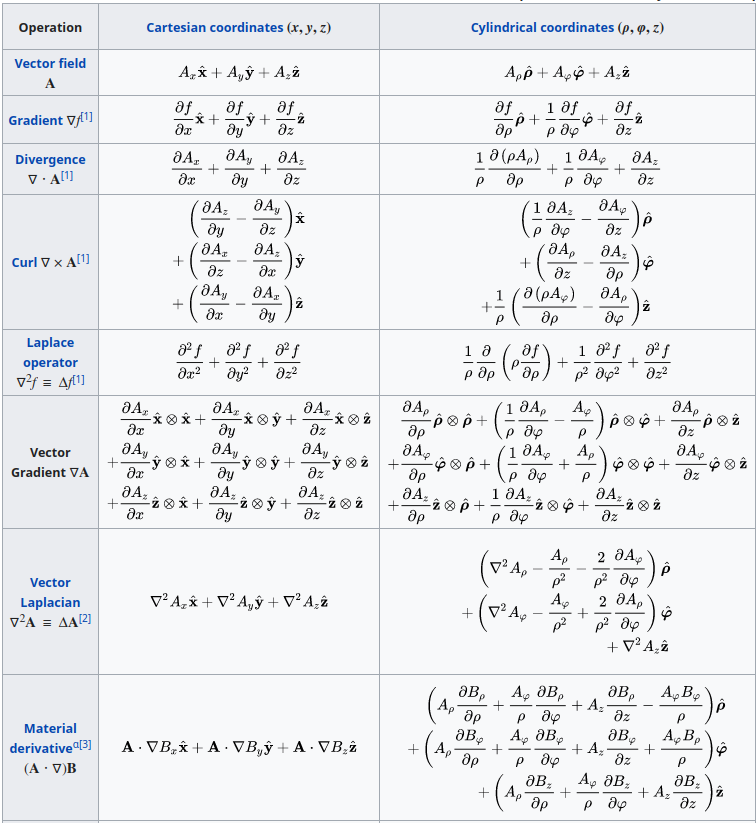
\includegraphics[scale=0.5]{DelInOtherCoordinateSystems.png}
  \caption{Del in Cartesian and Cylindrical Polar Coordinates. \underline{Source:} \url{https://en.wikipedia.org/wiki/Del_in_cylindrical_and_spherical_coordinates}}
  \label{fig:galaxy}
\end{figure}

\subsection{First-Order Linear ODE}
Equations of the form $\frac{dy}{dx} + \alpha(x) y = \beta(x)$ can be solved by multiplying both sides by an integrating factor $e^{\int_{}^{}\alpha(x)dx}$. Then the left-hand side becomes $\frac{d(e^{\int_{}^{}\alpha(x)dx}.y)}{dx}$ and the right hand side becomes $e^{\int_{}^{}\alpha(x)dx} \beta(x)$. The left and right hand sides can then be integrated directly.

\newpage
\section{Kinematics}

\subsection{Gauss' Divergence Theorem}
\begin{align*}
  \int_S \vec{b} . \hat{n} d A =  \int_S \vec{b} . \vec{d A} = \int_V \vec{\nabla} . \vec{b}\ d V
\end{align*}

\subsection{Stokes' Theorem}
\begin{align*}
  \oint_C \vec{b} . \vec{dl} =  \int_S (\vec{\nabla} \times \vec{b}) . \hat{n} d A = \int_S (\vec{\nabla} \times \vec{b}) . \vec{d A}
\end{align*}

\subsection{Streamlines, Pathlines, and Streaklines}
\begin{align*}
\text{Equations for Streamlines (Cartesian Coordinates) } \frac{dx}{v_x} &= \frac{dy}{v_y} = \frac{dz}{v_z} \\
\text{Equations for Streamlines (Cylindrical Polar Coordinates) } \frac{dr}{v_r} &= \frac{r d \theta}{v_\theta} = \frac{dz}{v_z} \\
\text{Equations for Pathlines (Cartesian Coordinates) } \frac{d x^M}{d t} &= v_x,\ \frac{d y^M}{d t} = v_y, \frac{d z^M}{d t} = v_z \\
\text{Equations for Pathlines (Cylindrical Polar Coordinates) } \frac{d r^M}{d t} &= v_r,\ r^M \frac{d \theta^M}{d t} = v_\theta, \frac{d z^M}{d t} = v_z \\
\text{Equations for Streaklines (Cartesian Coordinates) } \vec{r}^M(x, y, z, t=\tau) &= \vec{r}_\tau \text{ in pathline equations} \\
\text{Equations for Streaklines (Cylindrical Polar Coordinates) } \vec{r}^M(r, \theta, z, t=\tau) &= \vec{r}_\tau \text{ in pathline equations}
\end{align*}

\newpage
\section{Continuum Flow}
\subsection{Mass Conservation}
\begin{align*}
\frac{\partial \rho}{\partial t} + \vec{\nabla} . (\rho v_j) &= 0 \\
\frac{\partial \rho}{\partial t} + \frac{\partial (\rho v_j)}{\partial x_j} &= 0 \\
\end{align*}

\subsubsection{Cartesian Coordinates}
\begin{align*}
\frac{\partial \rho}{\partial t} + \frac{\partial (\rho v_1)}{\partial x_1} + \frac{\partial (\rho v_2)}{\partial x_2} + \frac{\partial (\rho v_3)}{\partial x_3} &= 0 \\
\end{align*}

\subsubsection{Cylindrical Polar Coordinates}
\begin{align*}
\frac{\partial \rho}{\partial t} + \frac{1}{r} \frac{\partial}{\partial r} (r \rho v_r) + \frac{1}{r} \frac{\partial \rho v_{\theta}}{\partial \theta} + \frac{\partial \rho v_z}{\partial z} &= 0 \\
\end{align*}

\subsection{Momentum Conservation (Navier-Stokes Equations)}
$\rho \biggl[\dfrac{\partial{\vec{v}}}{\partial t} + (\vec{v}.\vec{\nabla})\vec{v}\biggr] = \rho \vec{f} -\vec{\nabla} p + \mu \nabla^2 \vec{v}$

\subsubsection{Cartesian Coordinates}
\begin{align*}
\rho \biggl[ \frac{\partial v_1}{\partial t} + v_1 \frac{\partial v_1}{\partial x_1} + v_2 \frac{\partial v_1}{\partial x_2} + v_3 \frac{\partial v_1}{\partial x_3} \biggr] &= \rho f_1 - \frac{\partial p}{\partial x_1} + \mu \biggl[ \frac{\partial^2 v_1}{\partial x^2_1} + \frac{\partial^2 v_1}{\partial x^2_2} + \frac{\partial^2 v_1}{\partial x^2_3} \biggr] \\
\rho \biggl[ \frac{\partial v_2}{\partial t} + v_1 \frac{\partial v_2}{\partial x_1} + v_2 \frac{\partial v_2}{\partial x_2} + v_3 \frac{\partial v_2}{\partial x_3} \biggr] &= \rho f_2 - \frac{\partial p}{\partial x_2} + \mu \biggl[ \frac{\partial^2 v_2}{\partial x^2_1} + \frac{\partial^2 v_2}{\partial x^2_2} + \frac{\partial^2 v_2}{\partial x^2_3} \biggr] \\
\rho \biggl[ \frac{\partial v_3}{\partial t} + v_1 \frac{\partial v_3}{\partial x_1} + v_2 \frac{\partial v_3}{\partial x_2} + v_3 \frac{\partial v_3}{\partial x_3} \biggr] &= \rho f_3 - \frac{\partial p}{\partial x_3} + \mu \biggl[ \frac{\partial^2 v_3}{\partial x^2_1} + \frac{\partial^2 v_3}{\partial x^2_2} + \frac{\partial^2 v_3}{\partial x^2_3} \biggr] \\
\end{align*}

\subsubsection{Cylindrical Polar Coordinates}
\begin{mywideralign*}
\rho \biggl[ \frac{\partial v_r}{\partial t} + v_r \frac{\partial v_r}{\partial r} + \frac{v_{\theta}}{r} \frac{\partial v_r}{\partial \theta} + v_z \frac{\partial v_r}{\partial z} - \frac{{v^2}_{\theta}}{r} \biggr] &= \rho f_r - \frac{\partial p}{\partial r} + \mu \biggl[ \frac{\partial}{\partial r} \biggl( \frac{1}{r} \frac{\partial}{\partial r} ( r v_r ) \biggr) + \frac{1}{r^2} \frac{{\partial}^2 v_r}{\partial {\theta}^2} + \frac{{\partial}^2 v_r}{\partial z^2} -\frac{2}{r^2} \frac{\partial v_{\theta}}{\partial \theta}  \biggr] \\
\rho \biggl[ \frac{\partial v_{\theta}}{\partial t} + v_r \frac{\partial v_{\theta}}{\partial r} + \frac{v_{\theta}}{r} \frac{\partial v_{\theta}}{\partial \theta} + v_z \frac{\partial v_{\theta}}{\partial z} + \frac{v_r v_{\theta}}{r} \biggr] &= \rho f_{\theta} - \frac{1}{r} \frac{\partial p}{\partial \theta} + \mu \biggl[ \frac{\partial}{\partial r} \biggl( \frac{1}{r} \frac{\partial}{\partial r} ( r v_{\theta} ) \biggr) + \frac{1}{r^2} \frac{{\partial}^2 v_{\theta}}{\partial {\theta}^2} + \frac{{\partial}^2 v_{\theta}}{\partial z^2} +\frac{2}{r^2} \frac{\partial v_r}{\partial \theta}  \biggr] \\
\rho \biggl[ \frac{\partial v_z}{\partial t} + v_r \frac{\partial v_z}{\partial r} + \frac{v_{\theta}}{r} \frac{\partial v_z}{\partial \theta} + v_z \frac{\partial v_z}{\partial z} \biggr] &= \rho f_z - \frac{\partial p}{\partial z} + \mu \biggl[ \frac{1}{r} \frac{\partial}{\partial r} \biggl( r \frac{\partial v_z}{\partial r} \biggr) + \frac{1}{r^2} \frac{{\partial}^2 v_z}{\partial {\theta}^2} + \frac{{\partial}^2 v_z}{\partial z^2} \biggr]
\end{mywideralign*}

\subsection{Flow Conditions} 

\subsubsection{Steady State}
\begin{align*}
& \frac{\partial \rho}{\partial t} = 0, \\
& \frac{\partial v_1}{\partial t} = 0,\ \frac{\partial v_2}{\partial t} = 0,\ \frac{\partial v_3}{\partial t} = 0 
\end{align*}

\subsubsection{Fully Developed}
\begin{align*}
& \frac{\partial v_1}{\partial x_1} = 0,\ \frac{\partial v_2}{\partial x_2} = 0,\ \frac{\partial v_3}{\partial x_3} = 0
\end{align*}

\subsubsection{Unidirectional}
\begin{align*}
& v_{n1} = 0,\ v_{n2} = 0
\end{align*}

\subsubsection{Two-dimensional}
\begin{align*}
& v_{n} = 0,\\
&\frac{\partial v_{t1}}{\partial s_n} = 0,\ \frac{\partial v_{t2}}{\partial s_n} = 0
\end{align*}

\subsubsection{Free Surface}
\begin{align*}
& \frac{\partial p}{\partial s_t} =0
\end{align*}

\subsubsection{Axisymmetric}
\begin{align*}
& v_\theta = 0, \\
& \frac{\partial v_r}{\partial \theta} = 0,\ \frac{\partial v_\theta}{\partial \theta} = 0, \frac{\partial v_z}{\partial \theta} = 0,\\
\end{align*}

\subsubsection{\underline{Simple} Couette Flow}
\begin{align*}
\frac{\partial p}{\partial x_1} = 0,\ \frac{\partial p}{\partial x_2} = 0,\ \frac{\partial p}{\partial x_3} = 0 
\end{align*}

\subsection{Boundary Conditions} 
\textit{Let $t$ indicate a direction tangent to the boundary} \\
\textit{Let $n$ indicate a direction normal to the boundary}

\subsubsection{Fluid-Solid Interface}
\begin{align*}
\text{No Slip: } v_t\rvert_{boundary} = 0 \\
\text{No Penetration: } v_n\rvert_{boundary} = 0 \\
\end{align*}

\subsubsection{Fluid-Fluid Interface}
\begin{align*}
\text{Continuity:}& \ \rho_\Romannum{1} v_{\Romannum{1} n} = \rho_\Romannum{2} v_{\Romannum{2} n} \\
\text{Jump/Discontinuity:}& \ \rho_\Romannum{1} \neq \rho_\Romannum{2} \\
& v_{\Romannum{1} n} \neq v_{\Romannum{2} n} \\
\text{Shear Stress Continuity:}& \ T_{ij} n_j t_i \bigr\rvert_\Romannum{1} = T_{ij} n_j t_i \bigr\rvert_\Romannum{2} \\
& \implies \mu_\Romannum{1} \frac{\partial v_t}{\partial s_n} \biggr\rvert_\Romannum{1} = \mu_\Romannum{2} \frac{\partial v_t}{\partial s_n} \biggr\rvert_\Romannum{2}
\end{align*}

\subsubsection{Fluid-Gas Interface}
\begin{align*}
\text{Free Surface:}& \ p \rvert_{boundary} = p_{\infty} \\
\text{Traction-Free:}& \ \frac{\partial v_t}{\partial s_n} \biggr\rvert_{boundary} = 0 \\
\end{align*}

\newpage
\section{Vorticity Dynamics}
\begin{align*}
\text{Circulation } \Gamma &= \oint_{C}^{} \vec{v} . \vec{dl} = \int_{S}^{} \vec{\omega}.\hat{n}\ dA \\ 
\text{Average angular velocity } \bar{\Omega} &= \frac{\bar{u}_{\theta}}{a} \\ &= \frac{\oint_{C}^{} \vec{v}.\vec{dl}}{2 \pi a^2} =  \frac{\Gamma}{2 \pi a^2} \text{ (On a circle of radius } a\text{)} \\ &= \frac{{\omega}_j n_j}{2}\\
\text{For Irrotational Flow, } \Gamma &= 0,\ \vec{\omega} = 0 \\
\text{A vector field } \vec{\alpha} \text{ is considered solenoidal if } \vec{\nabla} . \vec{\alpha} &= 0 \\
\vec{\nabla}.\vec{\omega} &= \vec{\nabla}.(\vec{\nabla} \times \vec{v}) = 0 \\
\end{align*}

\subsection{Streamlines and Vortex Lines}
\begin{align*}
\text{Equations for Streamlines (Cartesian Coordinates) } \frac{dx}{u_x} &= \frac{dy}{u_y} = \frac{dz}{u_z} \\
\text{Equations for Streamlines (Cylindrical Polar Coordinates) } \frac{dR}{u_R} &= \frac{R d \phi}{u_\phi} = \frac{dz}{u_z} \\
\text{Equations for Vortex Lines (Cartesian Coordinates) } \frac{dx}{\omega_x} &= \frac{dy}{\omega_y} = \frac{dz}{\omega_z} \\
\end{align*}

\subsection{Terms}
\begin{itemize}
\item \textbf{Barotropic}: Density is a function of pressure only. $\dfrac{1}{\rho^2} \vec{\nabla} \rho \times \vec{\nabla} p = 0$ 
\item \textbf{Inviscid}: Viscosity can be neglected. $\nu \nabla^2 \vec{\omega} = 0$ 
\item \textbf{Baroclinic}: Measure of how misaligned the gradient of pressure is from the gradient of density in a fluid $\vec{\nabla} \rho \times \vec{\nabla} p$
\item \textbf{Isobars}: Constant pressure lines
\item \textbf{Isopycals}: Constant density lineses
\end{itemize}

\subsection{Vorticity Transport Equation}
\begin{align*}
\frac{D\vec{\omega}}{Dt} &= (\vec{\omega}.\vec{\nabla}) \vec{v} + \frac{1}{\rho^2} \vec{\nabla} \rho \times \vec{\nabla} p + \nu \nabla^2 \vec{\omega} \\
\frac{\partial \vec{\omega}}{\partial t} + (\vec{v}.\vec{\nabla})\vec{\omega} &= (\vec{\omega}.\vec{\nabla}) \vec{v} + \frac{1}{\rho^2} \vec{\nabla} \rho \times \vec{\nabla} p + \nu \nabla^2 \vec{\omega}
\end{align*}

\subsubsection{Legend}
\begin{itemize}
\item $\dfrac{D\vec{\omega}}{Dt}$: Total rate of change of vorticity of a fluid particle
\item $(\vec{\omega}.\vec{\nabla}) \vec{v}$: Vorticity production due to stretching/tilting of vortex lines
\item $\dfrac{1}{\rho^2} \vec{\nabla} \rho \times \vec{\nabla} p$: Vorticity production due to baroclinic effects
\item $\nu \nabla^2 \vec{\omega}$: Viscous diffusion of vorticity which dissipates or redistributes vorticity
\end{itemize}

\subsection{Helmholtz's Vortex Theorems for Inviscid Flows}
\subsubsection{Assumptions}
\begin{itemize}
\item Inviscid
\item Barotropic
\item Conservative Body Forces $\vec{F} = -\vec{\nabla{\psi}}$
\end{itemize}

\subsubsection{Statement}
\begin{itemize}
\item Fluid particles/element orignially free of vorticity remain free of vorticity (non-rotating)
\item Vortex lines (tubes) move with the fluid for inviscid flows. Vortex line is always comprised of the same fluid particles (Vorticity is frozen to the flow for inviscid flow)
\item The strength of the vortex tube (circulation) does not vary with time during the fluid motion. Vortex tubes must be closed, go to infinity, or end on solid boundaries.
\end{itemize}

\subsection{Kelvin's circulation theorem}
\subsubsection{Assumptions}
\begin{itemize}
\item Inviscid
\item Barotropic
\item Incompressible
\item Conservative Body Forces $\vec{F} = -\vec{\nabla{\psi}}$
\end{itemize}

\subsubsection{Statement}
The circulation (strength of the vortex) around a closed curve moving with the fluid will remain constant.

\begin{align*}
\frac{\partial \Gamma_C}{\partial t} + v_j \frac{\partial \Gamma_C}{\partial x_j} &= \oint_{C}^{} \nu \nabla^2\vec{v}.\vec{dx} \\
\text{For inviscid flow, } \frac{\partial \Gamma_C}{\partial t} + v_j \frac{\partial \Gamma_C}{\partial x_j} &= 0
\end{align*}

\subsection{Bernoulli's Equation}
\subsubsection{Assumptions}
\begin{itemize}
\item Inviscid $\nabla^2 v = 0$ $\rightarrow$ Euler
\item Only gravitational body forces (Conservative) $\rightarrow$ $f_i = -\dfrac{d \psi}{dx_i}$ where $\psi = g z$
\item Barotropic $\rightarrow$ $\rho = \rho(p)$
\item Steady flow $\rightarrow$ $\dfrac{\partial}{\partial t} = 0$ 
\end{itemize}
Note: No restriction on the compressiblity effects

\subsubsection{Statement}
\begin{align*}
\nabla \Biggl[\frac{\vec{v}.\vec{v}}{2} + g z + \int \frac{dp}{\rho} \Biggr] &= -\vec{\omega} \times \vec{v} \\
\text{Along streamline or vortex line } \frac{\vec{v}.\vec{v}}{2} + g z + \int \frac{dp}{\rho} &= \text{constant}\\
\text{Unsteady flow } \frac{\partial \phi}{\partial t} + \frac{\vec{v}.\vec{v}}{2} + g z + \int \frac{dp}{\rho} &= F(t)\\
\text{Steady Potential flow } \frac{\vec{v}.\vec{v}}{2} + g z + \int \frac{dp}{\rho} &= \text{constant throughout the flow}\\
\end{align*}

\newpage
\section{Potential Flow}
\begin{align*}
i &= \sqrt{-1} \\
z &= x + i y = r e^{i \theta} = r (\cos{\theta} + i \sin{\theta}) \\
\bar{z} &= x - i y = r e^{-i \theta} = r (\cos{\theta} - i \sin{\theta}) \\
x &= r \cos{\theta} \\
y &= r \sin{\theta} \\
r &= \sqrt{x^2 + y^2} = |z| = |z \bar{z}|^{\frac{1}{2}} \\
\theta &= arctan{\frac{y}{x}} \\
\text{2D Incompressible Potential Flow } \nabla^2 \phi &= 0 = \nabla^2 \psi \\
\text{Complex Potential\ } F(z) &= \phi(z) + i \psi(z) \\
\text{Complex Velocity\ } w(z) &= u - i v = (v_r - i v_{\theta}) e^{-i \theta} = \frac{dF(z)}{dz} \\
\bar{w}(z) &= u + i v = (v_r + i v_{\theta}) e^{i \theta} \\
\end{align*}


\subsection{Stream Function $\Leftrightarrow$ Potential Function $\Leftrightarrow$ Velocities}
Also called Cauchy Reimann Equations
\begin{align*}
u &= \frac{\partial \phi}{\partial x} = \frac{\partial \psi}{\partial y} \\
v &= \frac{\partial \phi}{\partial y} = -\frac{\partial \psi}{\partial x} \\ \\
v_r &= \frac{\partial \phi}{\partial r} = \frac{1}{r} \frac{\partial \psi}{\partial \theta} \\
v_{\theta} &= \frac{1}{r} \frac{\partial \phi}{\partial \theta} = -\frac{\partial \psi}{\partial r} \\
\end{align*}

\subsection{Cartesian $\Leftrightarrow$ Polar Velocities}
\begin{align*}
u &= v_r \cos{\theta} - v_{\theta} \sin{\theta} \\
v &= v_r \sin{\theta} + v_{\theta} \cos{\theta} \\ \\
v_r &= u \cos{\theta} + v \sin{\theta} \\
v_{\theta} &= -u \sin{\theta} + v \cos{\theta} \\
\end{align*}

\subsection{Complex Potentials}

\begin{landscape}

\begin{tabular}{|c|c|c|c|c|c|c|}
\hline & F(z) & $\phi$ & $\psi$ & w(z) & $u$ and $v_r$ & $v$ and $v_{\theta}$ \\

\hline \multirow{2}{*}{Uniform}
  & \multirow{2}{*}{$U e^{-i \alpha} z$} % F(z)
    & $U(x \cos{\alpha}+y \sin{\alpha})$ % phi(x,y)
    & $U(y \cos{\alpha}-x \sin{\alpha})$ % psi(x,y)
  & \multirow{2}{*}{$U e^{-i \alpha}$} % w(z)
    & $U \cos{\alpha}$ % u(x,y)
    & $U \sin{\alpha}$ % v(x,y)
  \\ \cline{3-4} \cline{6-7} 
  & 
    & $U r \cos(\theta - \alpha)$ % phi(r,theta)
    & $U r \sin(\theta - \alpha)$ % psi(r,theta)
  & 
    & $U \cos(\theta - \alpha)$ % v_r(r,theta)
    & $-U \sin(\theta - \alpha)$ % v_theta(r,theta)
\\

\hline \multirow{2}{*}{Corner}
  & \multirow{2}{*}{$C z^n$} % F(z)
    & % phi(x,y)
    & % psi(x,y)
  & \multirow{2}{*}{$n C z^{n-1}$} % w(z)
    & % u(x,y)
    & % v(x,y)
  \\ \cline{3-4} \cline{6-7} 
  & 
    & $C r^n \cos{n \theta}$ % phi(r,theta)
    & $C r^n \sin{n \theta}$ % psi(r,theta)
  & 
    & $n C r^{n-1} \cos[(n-1) \theta]$ % v_r(r,theta)
    & $- n C r^{n-1} \sin[(n-1) \theta]$ % v_theta(r,theta)
\\

\hline \multirow{2}{*}{Source/Sink}
  & \multirow{2}{*}{$\frac{m}{2 \pi} \ln(z - z_0)$} % F(z)
    & $\frac{m}{4 \pi} \ln[{x^2+y^2}]$ % phi(x,y)
    & $\frac{m}{2 \pi} \arctan{\frac{y}{x}}$ % psi(x,y)
  & \multirow{2}{*}{$\frac{m}{2 \pi (z - z_0)}$} % w(z)
    & $\frac{m}{2 \pi} \frac{x}{x^2+y^2}$ % u(x,y)
    & $\frac{m}{2 \pi} \frac{y}{x^2+y^2}$ % v(x,y)
  \\ \cline{3-4} \cline{6-7} 
  & 
    & $\frac{m}{2 \pi} \ln{r}$ % phi(r,theta)
    & $\frac{m}{2 \pi} \theta$ % psi(r,theta)
  & 
    & $\frac{m}{2 \pi r}$ % v_r(r,theta)
    & $0$ % v_theta(r,theta)
\\

\hline \multirow{2}{*}{Free Vortex} % Type
  & \multirow{2}{*}{$-\frac{i \Gamma}{2 \pi} \ln(z - z_0)$} % F(z)
    & $\frac{\Gamma}{2 \pi} \arctan{\frac{y}{x}}$ % phi(x,y)
    & $-\frac{\Gamma}{4 \pi} \ln[x^2 + y^2]$ % psi(x,y)
  & \multirow{2}{*}{$-\frac{i \Gamma}{2 \pi (z-z_0)}$} % w(z)
    & $-\frac{\Gamma}{2 \pi} \frac{y}{x^2 + y^2}$ % u(x,y)
    & $\frac{\Gamma}{2 \pi} \frac{x}{x^2 + y^2}$ % v(x,y)
  \\ \cline{3-4} \cline{6-7} 
  & 
    & $\frac{\Gamma}{2 \pi} \theta$ % phi(r,theta)
    & $-\frac{\Gamma}{2 \pi} \ln{r}$ % psi(r,theta)
  & 
    & $0$ % v_r(r,theta)
    & $\frac{\Gamma}{2 \pi r}$ % v_theta(r,theta)
\\

\hline \multirow{2}{*}{Dipole} % Type
  & \multirow{2}{*}{$\dfrac{\mu}{\pi z}$} % F(z)
    & $\frac{\mu}{\pi} \frac{x}{x^2+y^2}$ % phi(x,y)
    & $-\frac{\mu}{\pi} \frac{y}{x^2+y^2}$ % psi(x,y)
  & \multirow{2}{*}{$-\dfrac{\mu}{\pi z^2}$} % w(z)
    & $\frac{\mu}{\pi} \frac{y^2-x^2}{(x^2+y^2)^2}$ % u(x,y)
    & $-\frac{\mu}{\pi} \frac{2xy}{(x^2+y^2)^2}$ % v(x,y)
  \\ \cline{3-4} \cline{6-7} 
  & 
    & $\frac{\mu}{\pi r} \cos{\theta}$ % phi(r,theta)
    & $-\frac{\mu}{\pi r} \sin{\theta}$ % psi(r,theta)
  & 
    & $-\frac{\mu}{\pi r^2} \cos{\theta}$ % v_r(r,theta)
    & $-\frac{\mu}{\pi r^2} \sin{\theta}$ % v_theta(r,theta)
\\

% \hline \multirow{2}{*}{} % Type
%   & \multirow{2}{*}{$$} % F(z)
%     & $$ % phi(x,y)
%     & $$ % psi(x,y)
%   & \multirow{2}{*}{$$} % w(z)
%     & $$ % u(x,y)
%     & $$ % v(x,y)
%   \\ \cline{3-4} \cline{6-7} 
%   & 
%     & $$ % phi(r,theta)
%     & $$ % psi(r,theta)
%   & 
%     & $$ % v_r(r,theta)
%     & $$ % v_theta(r,theta)
% \\

\hline
\end{tabular}
 
\vspace{-4mm}

\subsubsection{Legend}
\setlist{topsep=0pt, leftmargin=*}
\begin{itemize}
  \item Uniform
  \begin{itemize}
    \item $U$: Uniform velocity magnitude
    \item $\alpha$: Angle of attack - the angle at which the direction of the uniform velocity is oriented with respect to the horizontal
  \end{itemize}
  \item Corner
  \begin{itemize}
    \item $C$: Indicates the direction. $C > 0$ always
    \item $n$: $\dfrac{\pi}{\text{angle of the corner}}$
  \end{itemize} 
  \item Source/Sink
  \begin{itemize}
    \item $m$: Volume flow rate per unit dimension normal to the page. For source, $m > 0$, whereas for sink, $m < 0$
  \end{itemize}
  \item Dipole/Doublet
  \begin{itemize}
    \item $a$: Half distance between the source and sink
    \item $Q$: Volume flow rate per unit dimension normal to the page
    \item $\mu$: $Q a$
  \end{itemize}        
\end{itemize}

\end{landscape}

\subsection{Infinite Series Expansions}
\begin{itemize}
  \item $\ln(1+\epsilon) = \epsilon - \frac{\epsilon^2}{2} + \frac{\epsilon^3}{3} - \dots$ when $|\epsilon| \le 1$
  \item $(1+\epsilon)^{-1} = 1 - \epsilon + \epsilon^2 - \epsilon^3 + \dots$ when $|\epsilon| \le 1$
  \item $(1+\epsilon)^{\frac{1}{2}} = 1 + \frac{1}{2} \epsilon - \frac{1}{8} \epsilon^2 + \frac{1}{16} \epsilon^3 - \frac{5}{128} \epsilon^4 + \frac{7}{256} \epsilon^5 - \dots$ when $|\epsilon| \le 1$
  \item $(1+\epsilon)^{-\frac{1}{2}} = 1 - \frac{1}{2} \epsilon + \frac{3}{8} \epsilon^2 - \frac{5}{16} \epsilon^3 + \frac{35}{128} \epsilon^4 - \frac{63}{256} \epsilon^5 + \dots$ when $|\epsilon| \le 1$
  \item $e^{\epsilon} = 1 - \frac{\epsilon^2}{2!} + \frac{\epsilon^4}{4!} - \dots$
  \item $\sin(\epsilon) = \epsilon - \frac{\epsilon^3}{3!} + \frac{\epsilon^5}{5!} - \frac{\epsilon^7}{7!} + \dots$ 
\end{itemize}

\subsection{Bernoulli's Equation (Irrotational)}
$p_{\infty} + \dfrac{\rho v^2_{\infty}}{2} = p + \dfrac{\rho |v^2|}{2} $

\subsection{Forces on a 2D Body}
\textit{All the below forces have the units of Force per unit length normal to the sheet of paper}
\begin{align*}
\text{Drag Force} &= -\int_{C}^{} (p-p_{\infty}) \cos{\theta}\ ds \\
\text{Lift Force} &= -\int_{C}^{} (p-p_{\infty}) \sin{\theta}\ ds \\
\text{Complex Force } G = D - i L &= -i \oint_{C}^{} p d\bar{z} = -i \oint_{C}^{} \Biggl[ p_{\infty} + \dfrac{\rho v^2_{\infty}}{2} -  \frac{\rho |v^2|}{2} \Biggr] d\bar{z} \\
&= \frac{i \rho}{2} \oint_{C}^{} |v^2| d\bar{z} = \frac{i \rho}{2} \oint_{C}^{} w \bar{w} d\bar{z} \\
&= \frac{i \rho}{2} \oint_{C}^{} [w(z)]^2 dz \ \bigl(\text{First Blasius Integral Law}\bigr) \\
\end{align*}

\subsection{Moment on a 2D Body}
\begin{align*}
\text{Moment } M &= -\dfrac{\rho}{2} Re \Biggl\{ \oint_{C}^{} z w^2 dz \Biggr\} \bigl(\text{Second Blasius Integral Law}\bigr) \\
\end{align*}

\subsection{Residue Theorem}
\begin{align*}
\text{If } F(z) &= \sum_{j}^{} \frac{B_j}{z - z_j} \\
R_k = \sum B \\
\oint_{C}^{} F(z) dz &= 2 \pi i \sum_{k}^{} R_k \\
\end{align*}

\newpage
\section{Boundary Layer Theory}
\begin{align*}
\text{Through dimensional analysis,} \\
\frac{\delta}{L} \sim \sqrt{\frac{\nu}{v L}} \sim \frac{1}{\sqrt{Re_L}} \\
\end{align*}

\subsection{Prandtl Boundary Layer Equations for a Flat Plate}
\begin{align*}
& \frac{\partial u}{\partial x} + \frac{\partial v}{\partial y} = 0 \\
& \rho \Biggl(u \frac{\partial u}{\partial x} + v \frac{\partial u}{\partial y} \Biggr) = -\frac{\partial p}{\partial x} + \mu \frac{{\partial}^2 u}{\partial y^2} \\
&\implies u \frac{\partial u}{\partial x} + v \frac{\partial u}{\partial y} = -\frac{1}{\rho} \frac{\partial p}{\partial x} + \nu \frac{{\partial}^2 u}{\partial y^2} \\
&\frac{\partial p}{\partial y} = 0
\end{align*}

\subsection{Blasius Solution for Boundary Layer for a Flat Plate}
This is a first order approximation for the steady, laminar, 2D boundary layer for a semi-infinite flat plate parallel to a constant, unidirectional flow where the pressure gradient $\dfrac{\partial p}{\partial t} = 0$.
\begin{align*}
\delta_{99} \approx \delta_v &\approx 5.29 \sqrt{\frac{\nu s_t}{u_\infty}} \\
\delta^* &= 1.72 \sqrt{\frac{\nu s_t}{u_\infty}} \\
\theta &= 0.665 \sqrt{\frac{\nu s_t}{u_\infty}} \\
\tau_w &= 0.332 \sqrt{\frac{\rho \mu u^3_\infty}{s_t}} \\
F \text{(one side of the plate) } &= 1.328 \sqrt{\rho \mu l u^3_\infty}
\end{align*}

\subsection{Common Viscosities}
\begin{itemize}
  \item Air: $\nu_{air} = 1.48 \times 10^{-5} m^2/s$ ($14.8\ centistokes$) \\
  \item Water: $\nu_{water} = 1 \times 10^{-6} m^2/s$ ($1\ centistoke$)
\end{itemize}

\subsection{Inviscid Equivalence}
\subsubsection{Displacement Thickness}
\begin{align*}
& \text{Decrease in flow-rate due to viscous flow vs inviscid flow} \\
& \text{(per unit length perpendicular to the plane)} \\
&= \int_A u_\infty dy dx - \int_A u dy dx = \int_A (u_\infty - u) dy dx \\
&= \int_0^\infty (u_\infty-u) dy = u_\infty \delta^* \\
& \implies \boxed{\delta^* = \int_0^\infty \biggl(1-\frac{u}{u_\infty} \biggr) dy}
\end{align*}

\subsubsection{Momentum Thickness}
\begin{align*}
& \text{Decrease in momentum flux due to viscous flow vs inviscid flow} \\
& \text{(per unit length in the z-direction)} \\
&= \int_A \rho u_\infty u \ dy dx - \int_A \rho u u \ dy dx = \int_A \rho (u_\infty - u) u\ dy dx \\
&= \int_0^\infty \rho (u_\infty-u) u \ dy = \rho u^2_\infty \theta \\
& \implies \boxed{\theta = \int_0^\infty \frac{u}{u_\infty} \biggl(1-\frac{u}{u_\infty} \biggr) dy}
\end{align*}

\subsubsection{Von Karman Momentum Integral Equation}
\begin{align*}
\frac{d}{d x} (\tilde{v}^2 \theta) &+ \tilde{v} \frac{d \tilde{v}}{dx} \delta^* = \frac{\tau_w}{\rho} \\
\text{where, }& \\
& \delta^* \text{ is the displacement thickness} \\
& \theta \text{ is the momentum thickness} \\
& \tilde{v}(x) = u \rvert_{boundary\ layer\ edge} \\
& \tau_w = \mu \frac{\partial u}{\partial y} \biggr\rvert_{y=0}
\end{align*}

\underline{Special Case}: If $\tilde{v} = u_{\infty} = constant$,
\begin{align*}
\text{Shear Stress on the plate } \tau_w &= \rho u_{\infty}^2 \frac{d \theta}{d x} \\
\text{Force on the plate } F = \int \tau_w dx &= \rho u_{\infty}^2 \theta \\
\text{Skin Friction Coefficient } C_f = \dfrac{\tau_w}{\biggl(\dfrac{\rho u_{\infty}^2}{2}\biggr)} &= 2 \frac{d \theta}{d x}
\end{align*}

\subsubsection{Momentum Equation at the Cylindrical Surface}
\begin{align*}
\mu \frac{\partial^2 u}{\partial y^2} = \frac{\partial p}{\partial x} = - \rho \tilde{v} \frac{\partial \tilde{v}}{\partial x}
\end{align*}

\subsubsection{Boundary Layer Separation Point}
\begin{align*}
\frac{\partial u}{\partial y} \biggr\rvert_{y=0} = 0
\end{align*}

\subsubsection{Shape Factor}
The higher the shape factor $\dfrac{\delta^*}{\theta}$, the closer a flow is towards separation

\end{document}
